\documentclass[a4paper, 11pt]{article}
\usepackage[a4paper, margin=1.5cm]{geometry}
\usepackage{graphicx}

\begin{document}

\clearpage\section*{Time to five minutes}

\subsection*{Problem Set \textnumero 1}

Write the time in words, to the nearest five minutes.

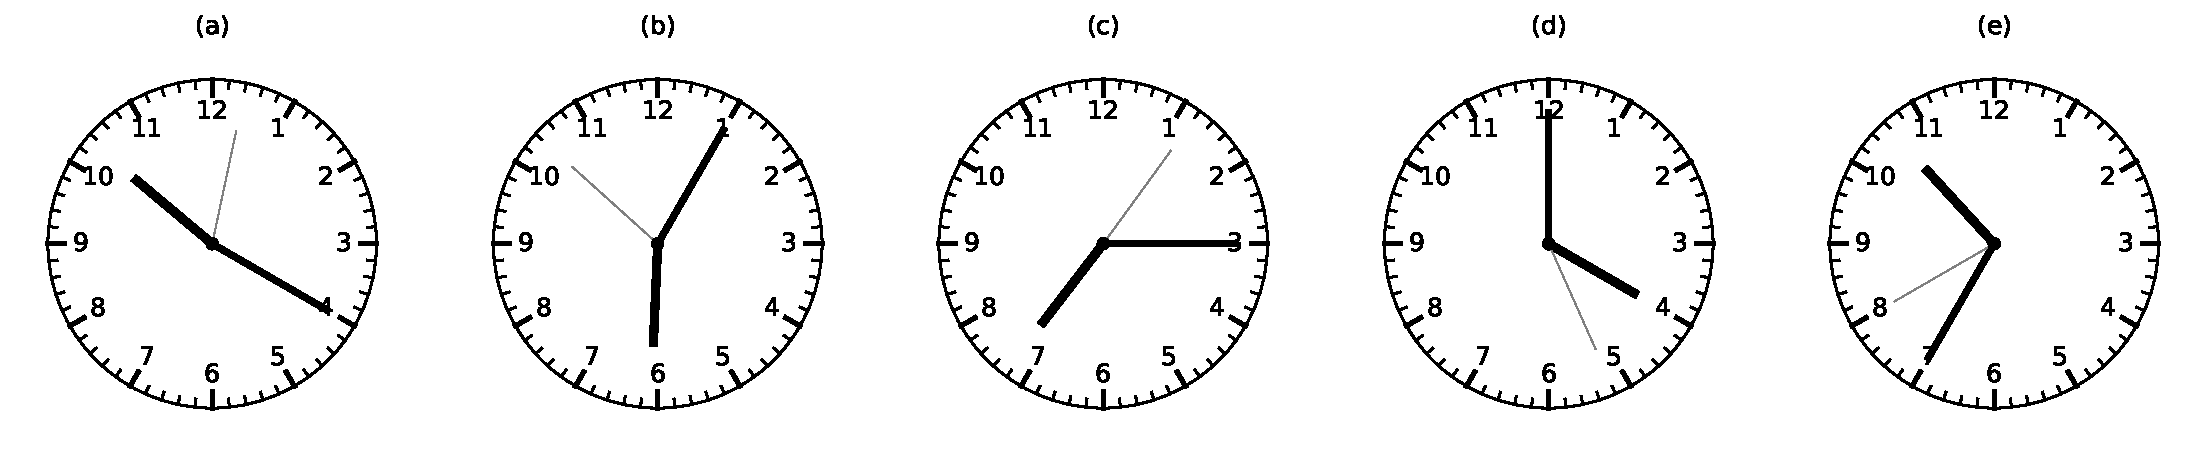
\includegraphics[width=\textwidth]{time/clocks_1_0.pdf}
\begin{enumerate}\item[(a)] \dotfill\bigskip
\item[(b)] \dotfill\bigskip
\item[(c)] \dotfill\bigskip
\item[(d)] \dotfill\bigskip
\item[(e)] \dotfill\bigskip
\end{enumerate}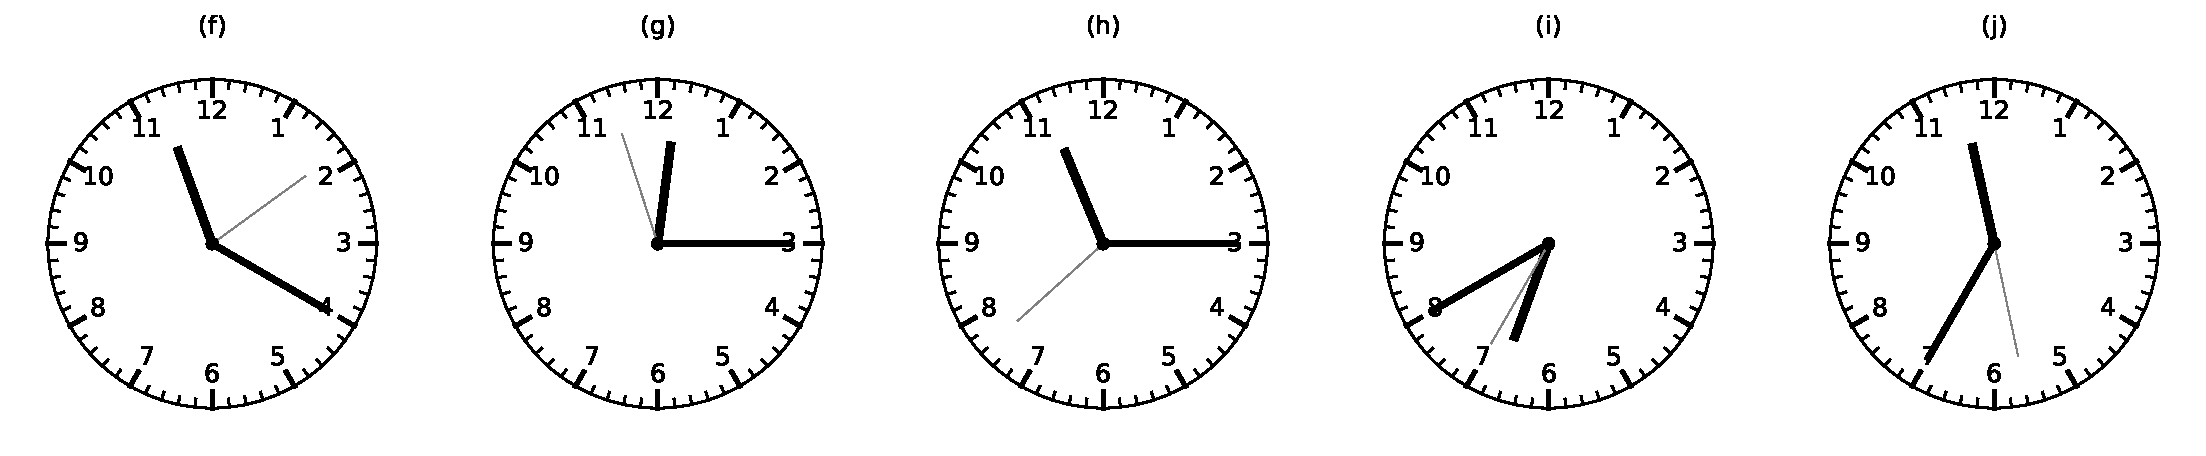
\includegraphics[width=\textwidth]{time/clocks_1_1.pdf}
\begin{enumerate}\item[(f)] \dotfill\bigskip
\item[(g)] \dotfill\bigskip
\item[(h)] \dotfill\bigskip
\item[(i)] \dotfill\bigskip
\item[(j)] \dotfill\bigskip
\end{enumerate}\clearpage
\subsection*{Problem Set \textnumero 2}

Write the time in words, to the nearest five minutes.

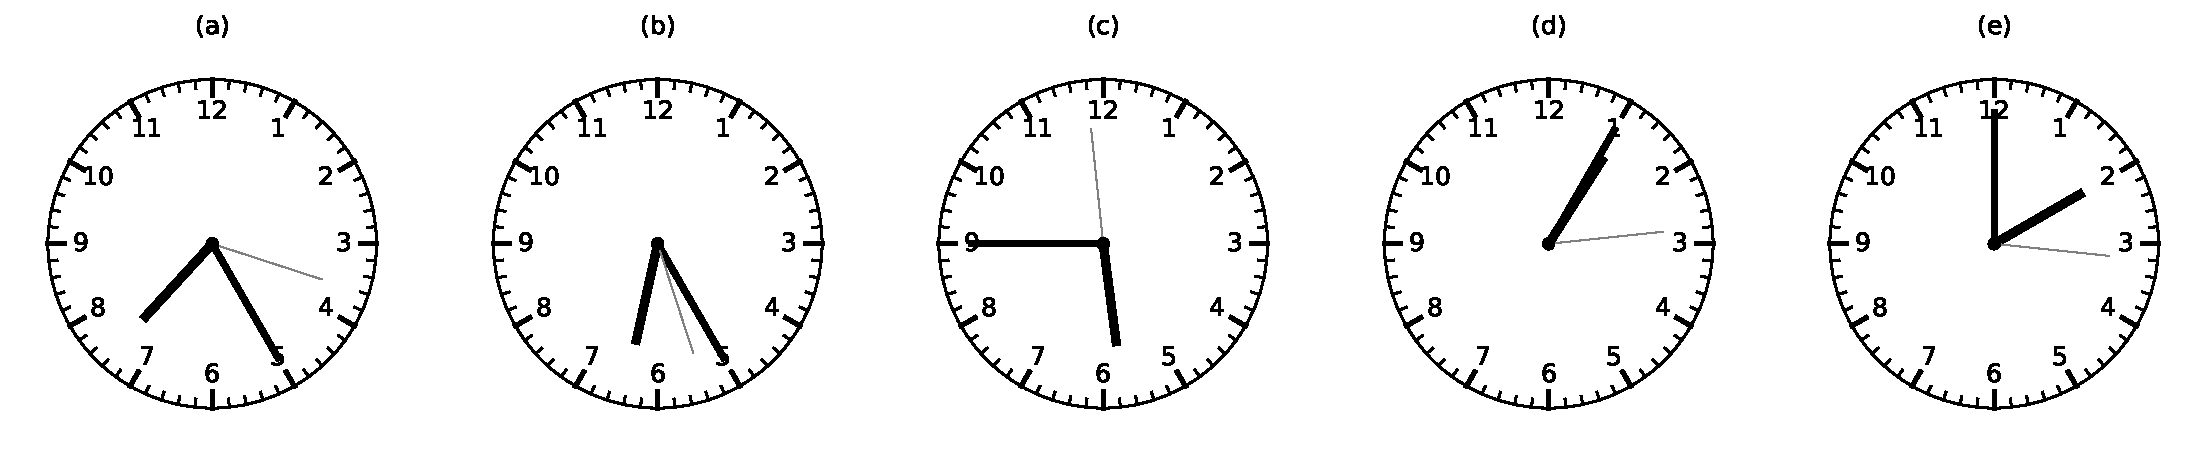
\includegraphics[width=\textwidth]{time/clocks_2_0.pdf}
\begin{enumerate}\item[(a)] \dotfill\bigskip
\item[(b)] \dotfill\bigskip
\item[(c)] \dotfill\bigskip
\item[(d)] \dotfill\bigskip
\item[(e)] \dotfill\bigskip
\end{enumerate}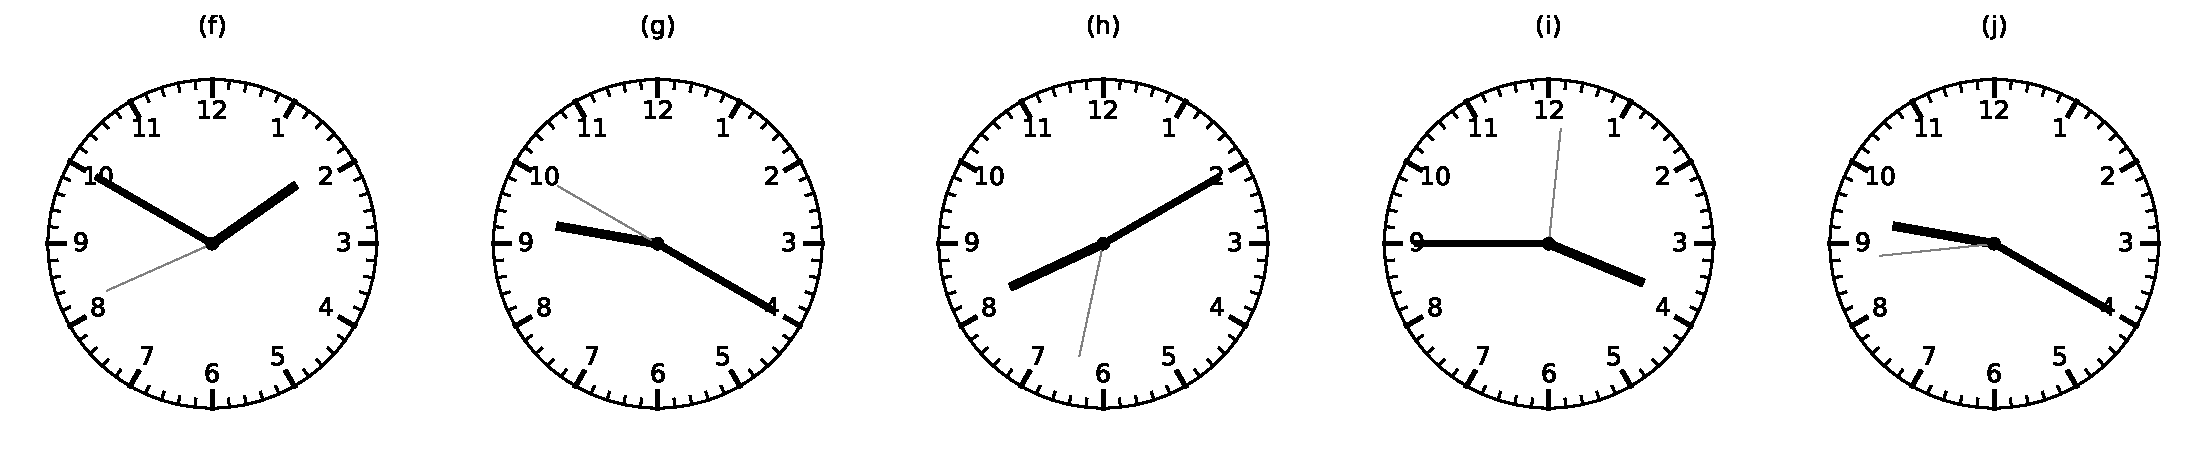
\includegraphics[width=\textwidth]{time/clocks_2_1.pdf}
\begin{enumerate}\item[(f)] \dotfill\bigskip
\item[(g)] \dotfill\bigskip
\item[(h)] \dotfill\bigskip
\item[(i)] \dotfill\bigskip
\item[(j)] \dotfill\bigskip
\end{enumerate}\clearpage
\subsection*{Problem Set \textnumero 3}

Write the time in words, to the nearest five minutes.

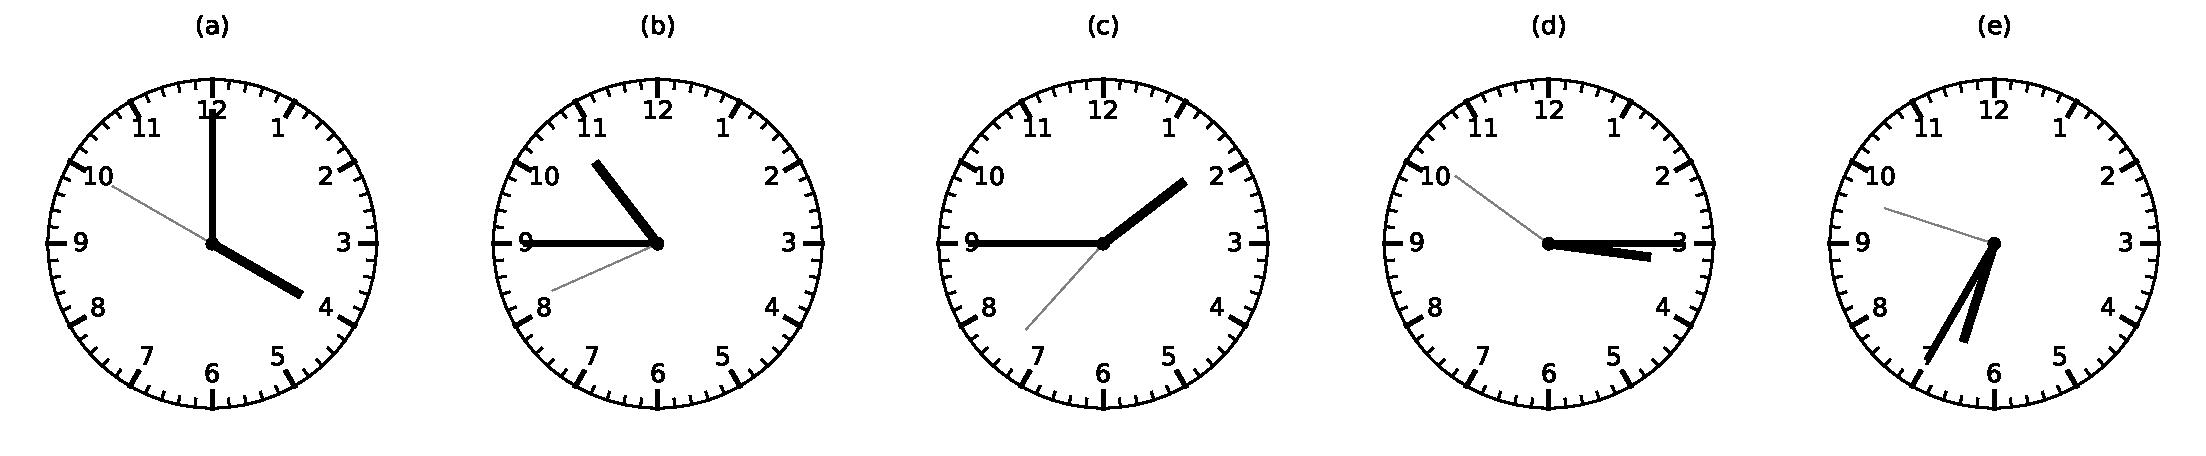
\includegraphics[width=\textwidth]{time/clocks_3_0.pdf}
\begin{enumerate}\item[(a)] \dotfill\bigskip
\item[(b)] \dotfill\bigskip
\item[(c)] \dotfill\bigskip
\item[(d)] \dotfill\bigskip
\item[(e)] \dotfill\bigskip
\end{enumerate}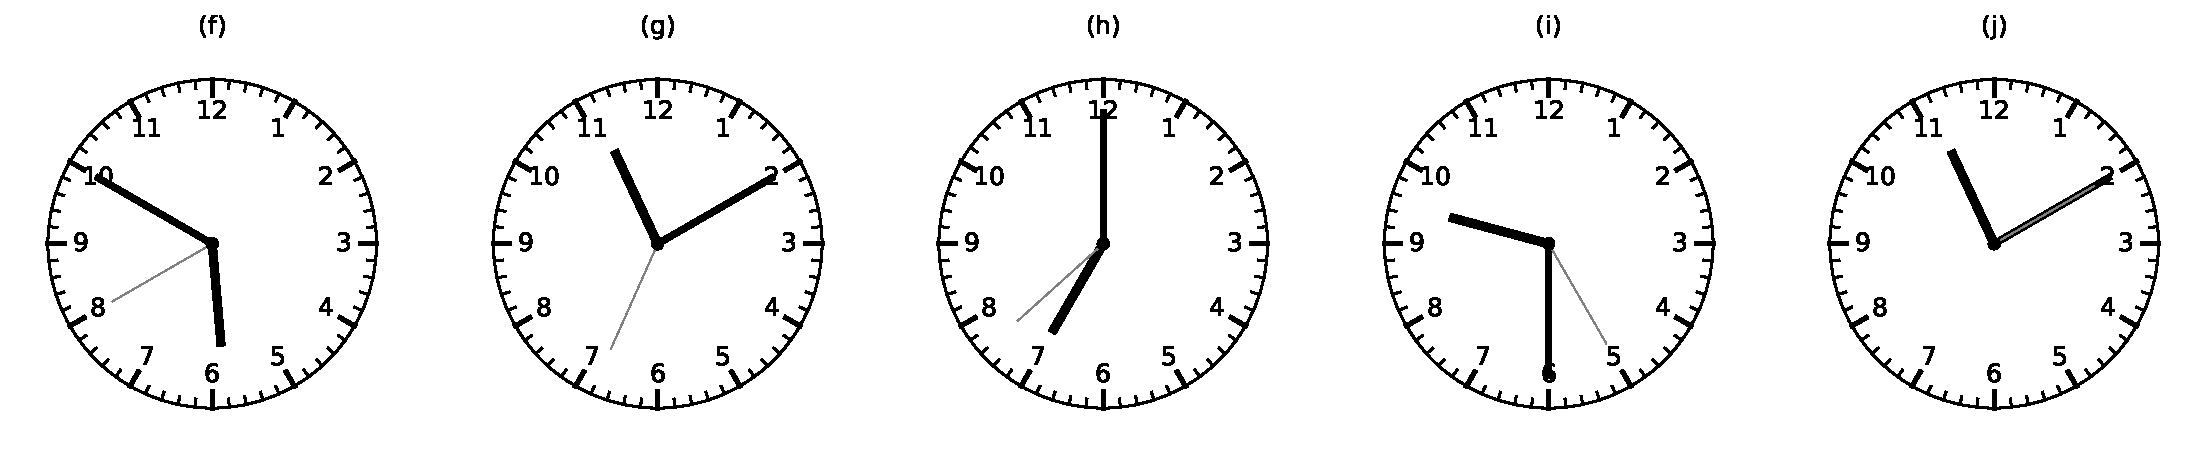
\includegraphics[width=\textwidth]{time/clocks_3_1.pdf}
\begin{enumerate}\item[(f)] \dotfill\bigskip
\item[(g)] \dotfill\bigskip
\item[(h)] \dotfill\bigskip
\item[(i)] \dotfill\bigskip
\item[(j)] \dotfill\bigskip
\end{enumerate}\clearpage
\subsection*{Problem Set \textnumero 4}

Write the time in words, to the nearest five minutes.

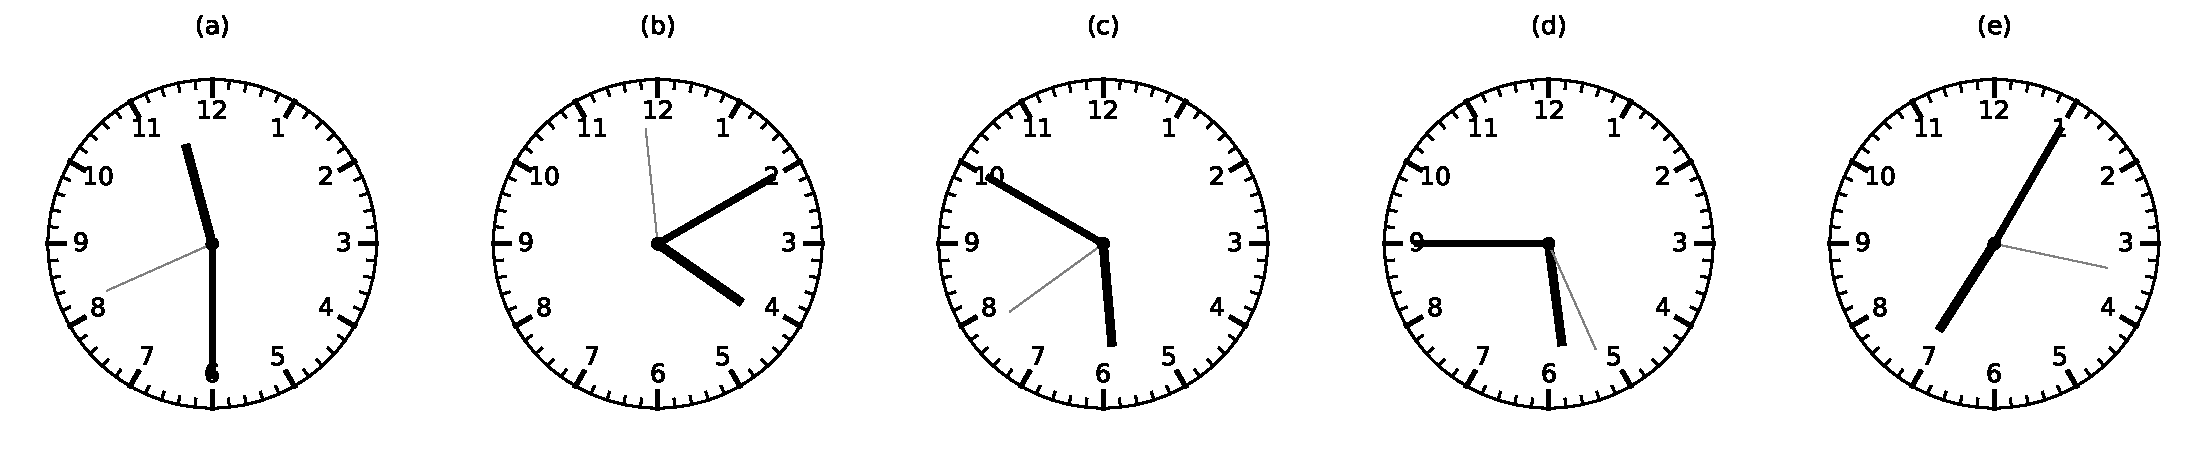
\includegraphics[width=\textwidth]{time/clocks_4_0.pdf}
\begin{enumerate}\item[(a)] \dotfill\bigskip
\item[(b)] \dotfill\bigskip
\item[(c)] \dotfill\bigskip
\item[(d)] \dotfill\bigskip
\item[(e)] \dotfill\bigskip
\end{enumerate}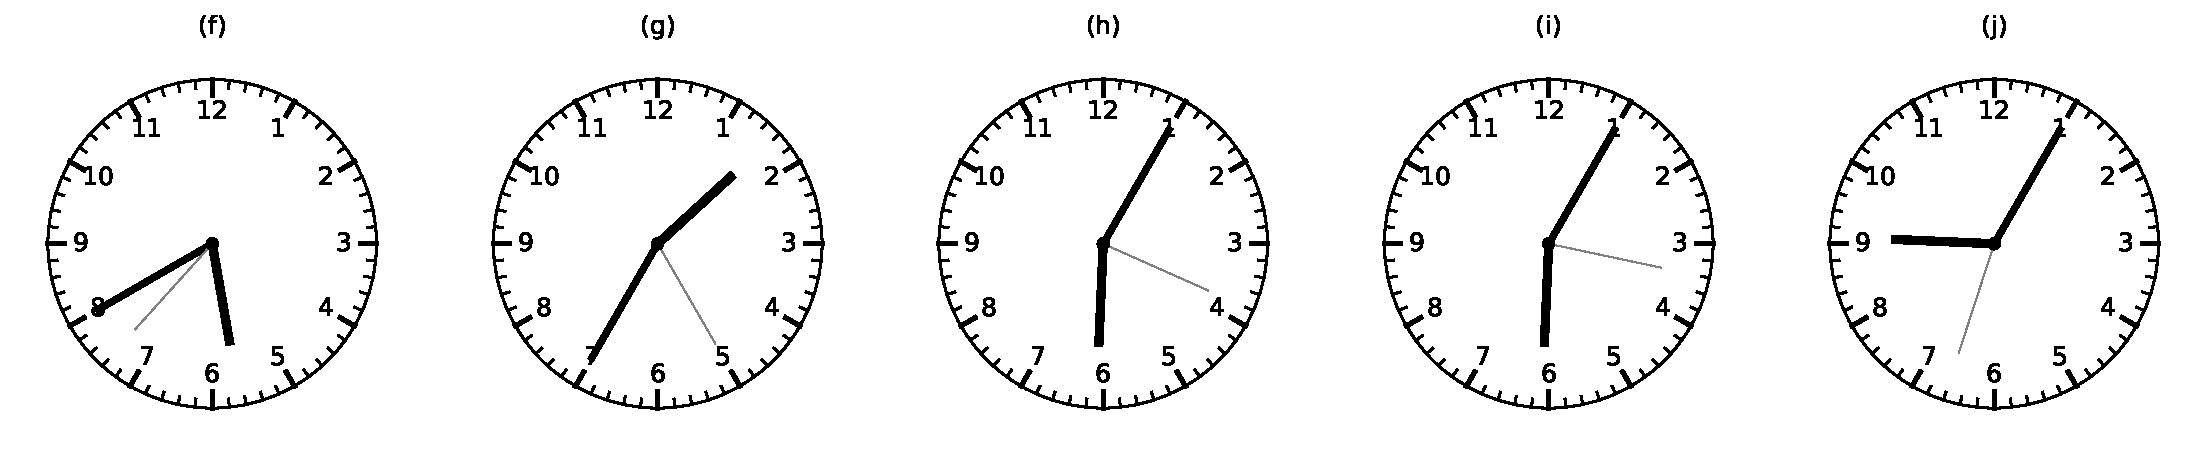
\includegraphics[width=\textwidth]{time/clocks_4_1.pdf}
\begin{enumerate}\item[(f)] \dotfill\bigskip
\item[(g)] \dotfill\bigskip
\item[(h)] \dotfill\bigskip
\item[(i)] \dotfill\bigskip
\item[(j)] \dotfill\bigskip
\end{enumerate}\clearpage
\subsection*{Problem Set \textnumero 5}

Write the time in words, to the nearest five minutes.

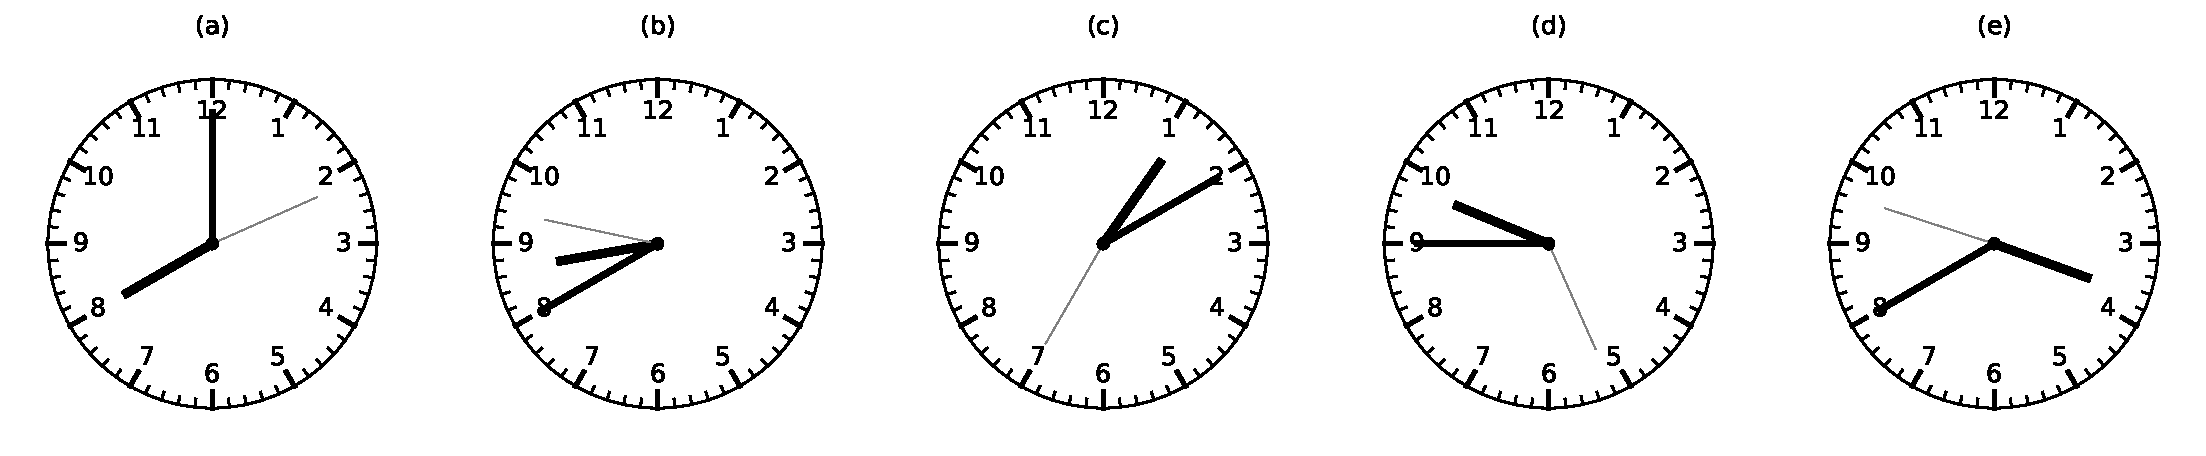
\includegraphics[width=\textwidth]{time/clocks_5_0.pdf}
\begin{enumerate}\item[(a)] \dotfill\bigskip
\item[(b)] \dotfill\bigskip
\item[(c)] \dotfill\bigskip
\item[(d)] \dotfill\bigskip
\item[(e)] \dotfill\bigskip
\end{enumerate}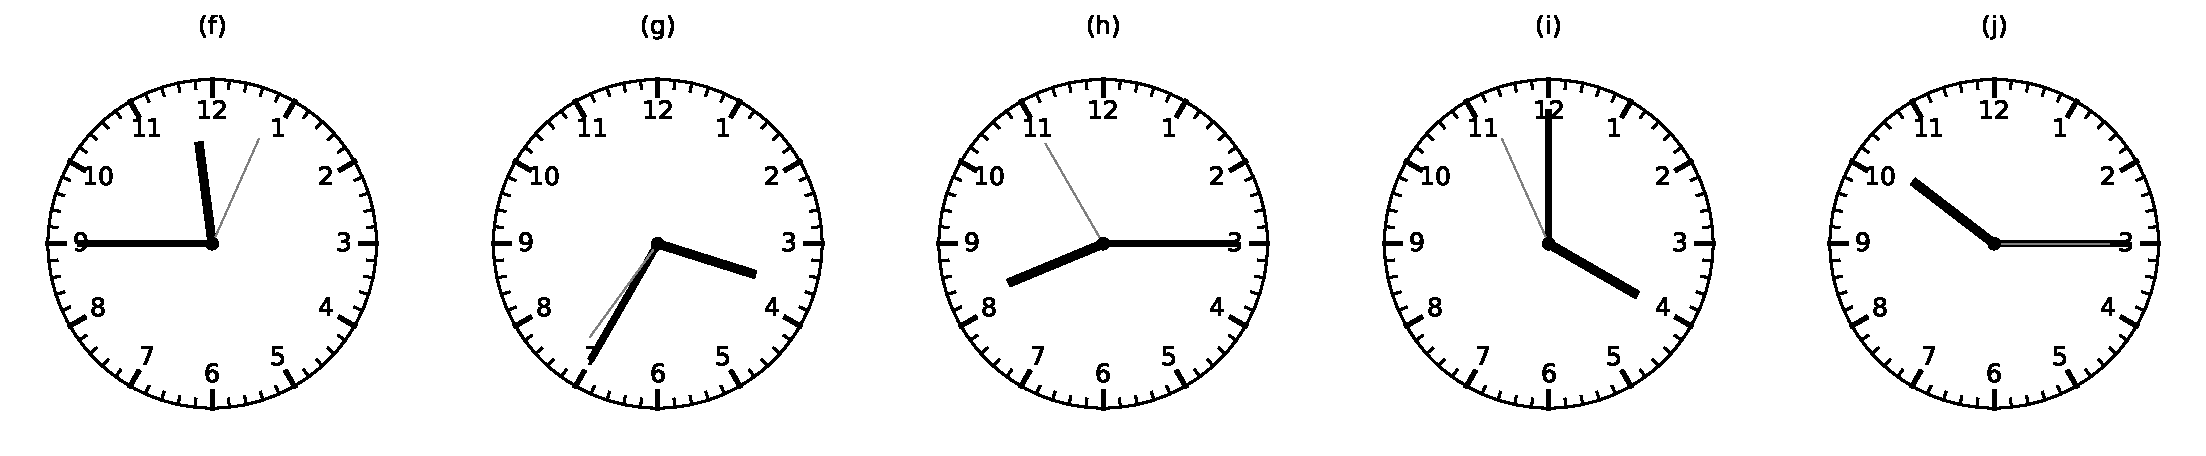
\includegraphics[width=\textwidth]{time/clocks_5_1.pdf}
\begin{enumerate}\item[(f)] \dotfill\bigskip
\item[(g)] \dotfill\bigskip
\item[(h)] \dotfill\bigskip
\item[(i)] \dotfill\bigskip
\item[(j)] \dotfill\bigskip
\end{enumerate}\clearpage\section*{Time to the minute}

\subsection*{Problem Set \textnumero 6}

Write the time in words, to the nearest minute. For example, ``twenty-three minutes past four."

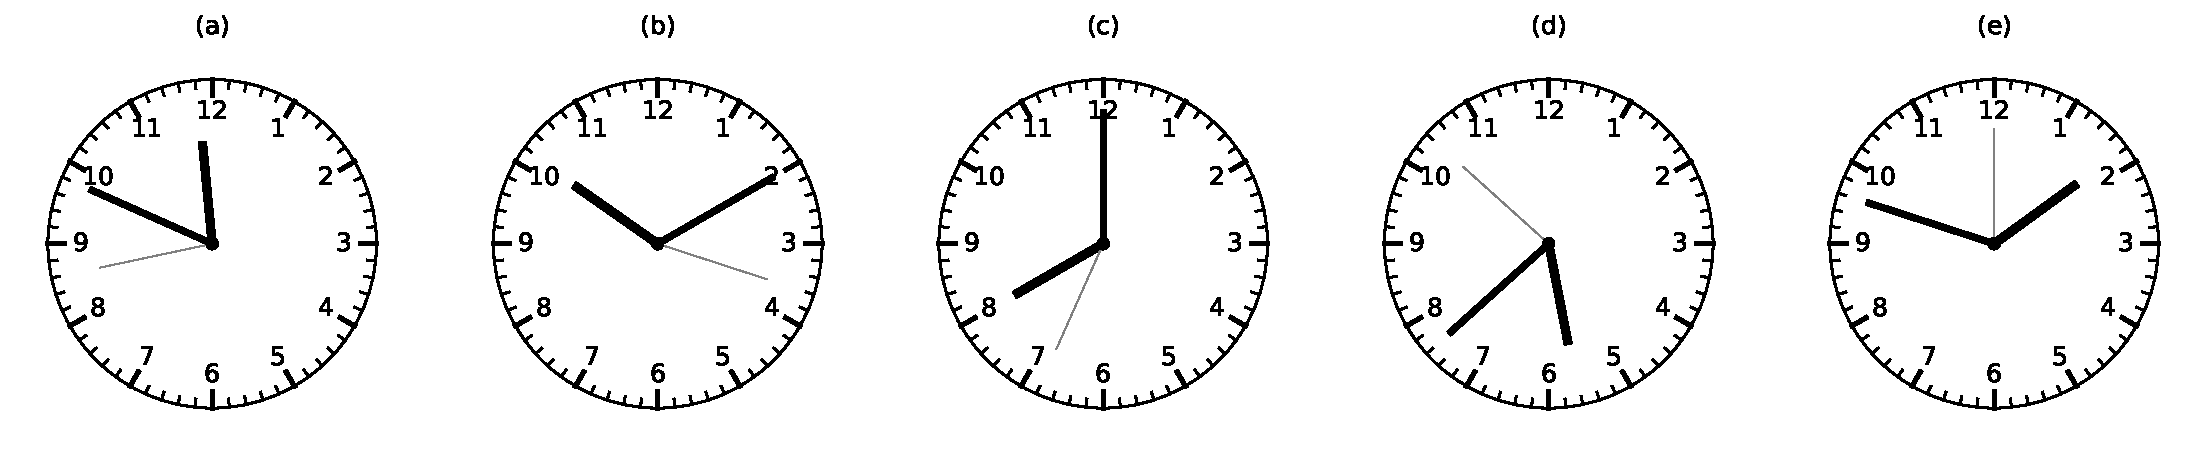
\includegraphics[width=\textwidth]{time/clocks_6_0.pdf}
\begin{enumerate}\item[(a)] \dotfill\bigskip
\item[(b)] \dotfill\bigskip
\item[(c)] \dotfill\bigskip
\item[(d)] \dotfill\bigskip
\item[(e)] \dotfill\bigskip
\end{enumerate}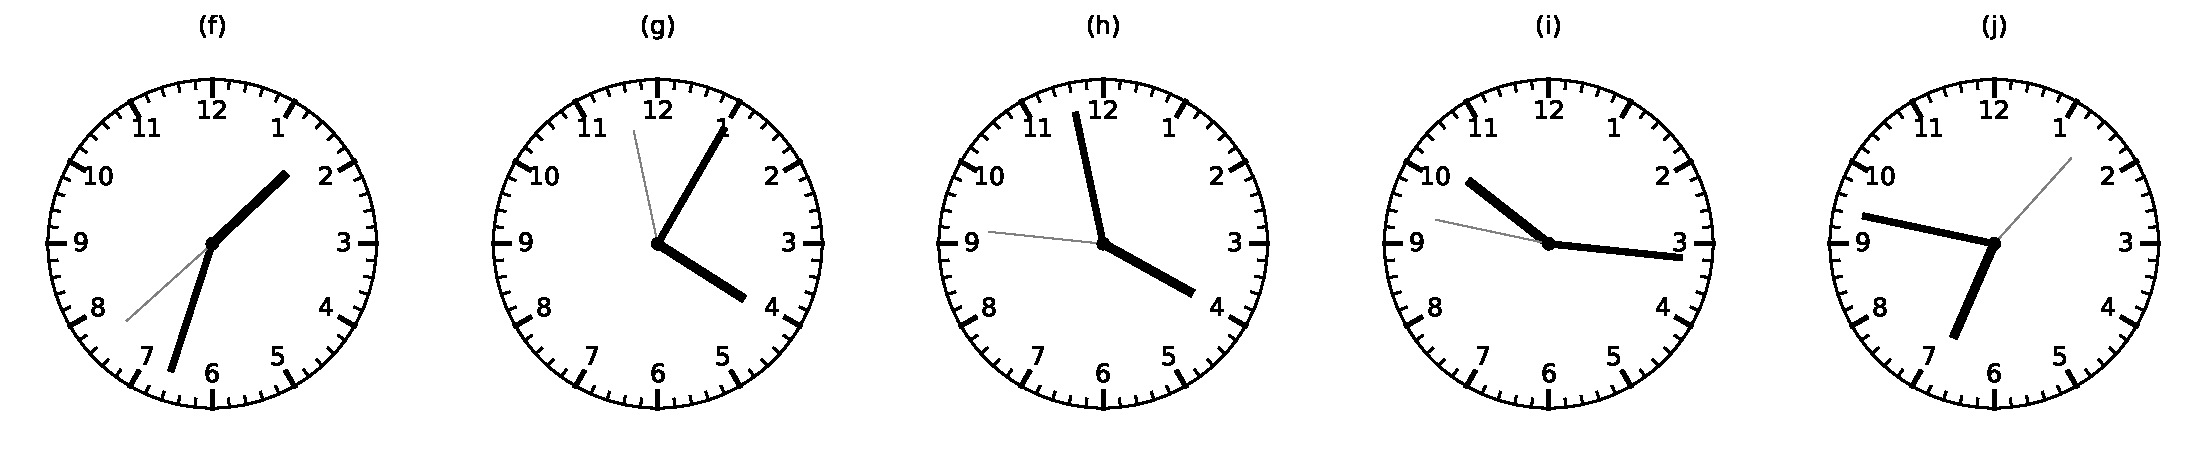
\includegraphics[width=\textwidth]{time/clocks_6_1.pdf}
\begin{enumerate}\item[(f)] \dotfill\bigskip
\item[(g)] \dotfill\bigskip
\item[(h)] \dotfill\bigskip
\item[(i)] \dotfill\bigskip
\item[(j)] \dotfill\bigskip
\end{enumerate}\clearpage
\subsection*{Problem Set \textnumero 7}

Write the time in words, to the nearest minute. For example, ``twenty-three minutes past four."

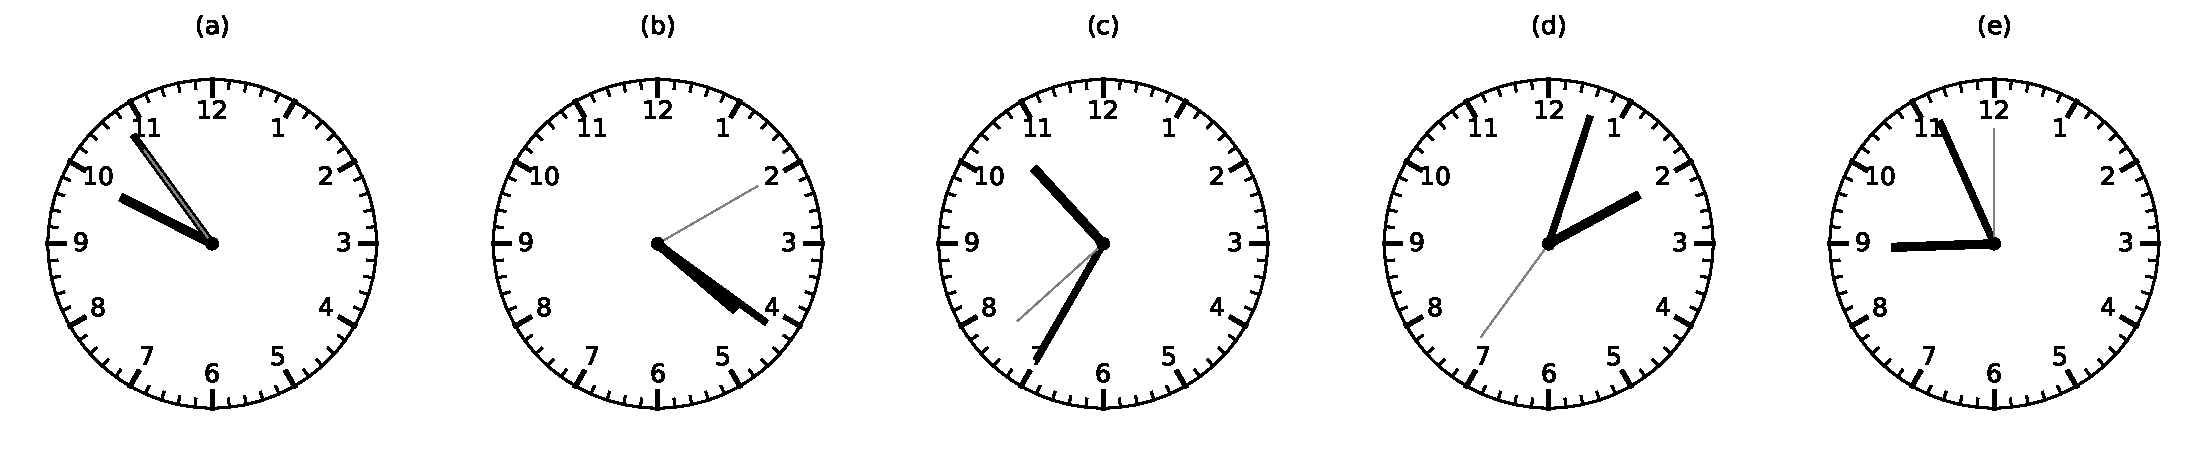
\includegraphics[width=\textwidth]{time/clocks_7_0.pdf}
\begin{enumerate}\item[(a)] \dotfill\bigskip
\item[(b)] \dotfill\bigskip
\item[(c)] \dotfill\bigskip
\item[(d)] \dotfill\bigskip
\item[(e)] \dotfill\bigskip
\end{enumerate}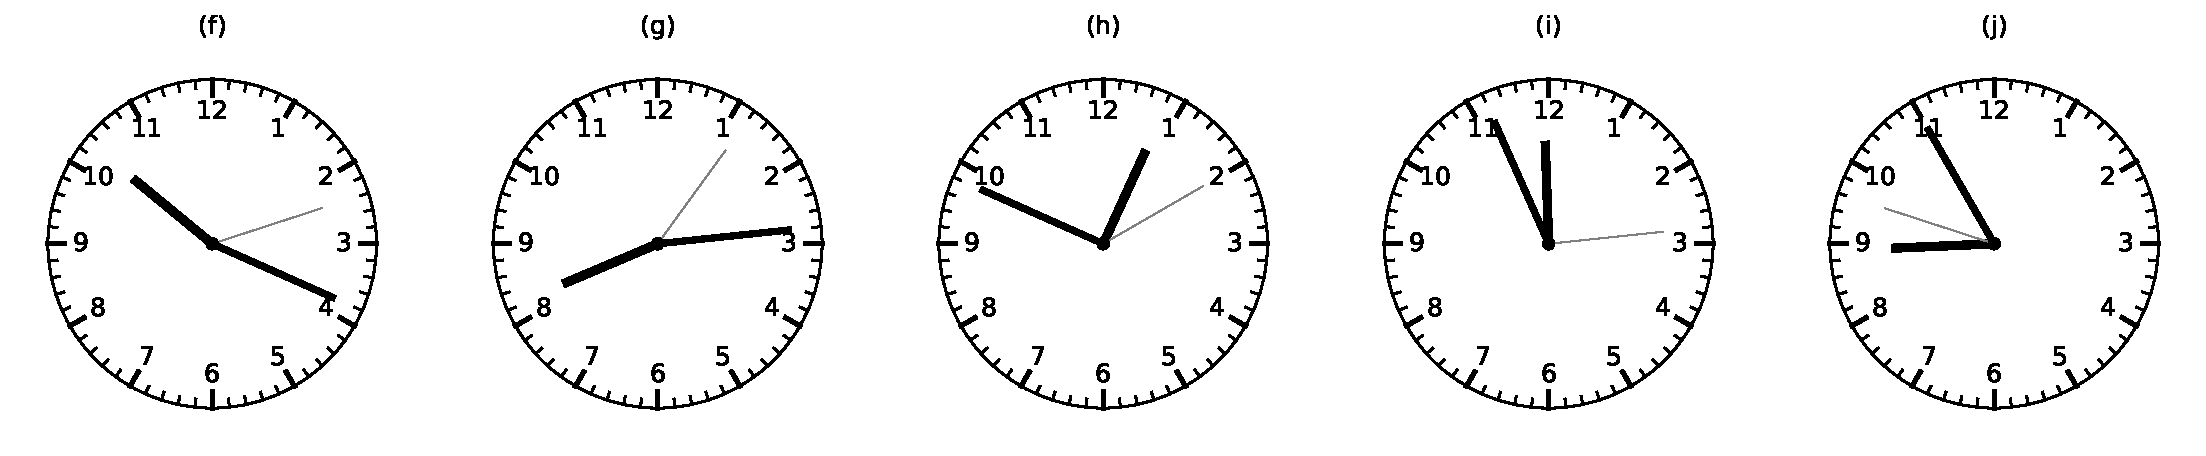
\includegraphics[width=\textwidth]{time/clocks_7_1.pdf}
\begin{enumerate}\item[(f)] \dotfill\bigskip
\item[(g)] \dotfill\bigskip
\item[(h)] \dotfill\bigskip
\item[(i)] \dotfill\bigskip
\item[(j)] \dotfill\bigskip
\end{enumerate}\clearpage
\subsection*{Problem Set \textnumero 8}

Write the time in words, to the nearest minute. For example, ``twenty-three minutes past four."

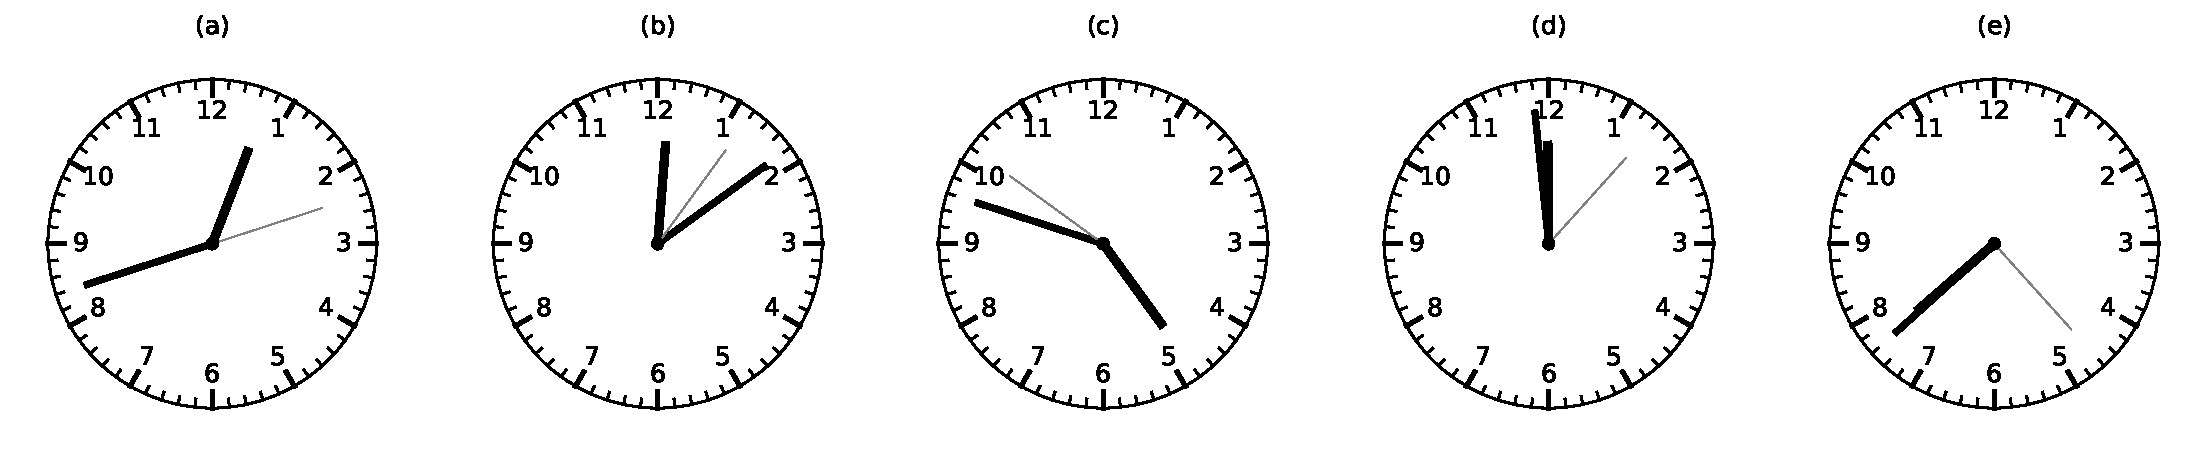
\includegraphics[width=\textwidth]{time/clocks_8_0.pdf}
\begin{enumerate}\item[(a)] \dotfill\bigskip
\item[(b)] \dotfill\bigskip
\item[(c)] \dotfill\bigskip
\item[(d)] \dotfill\bigskip
\item[(e)] \dotfill\bigskip
\end{enumerate}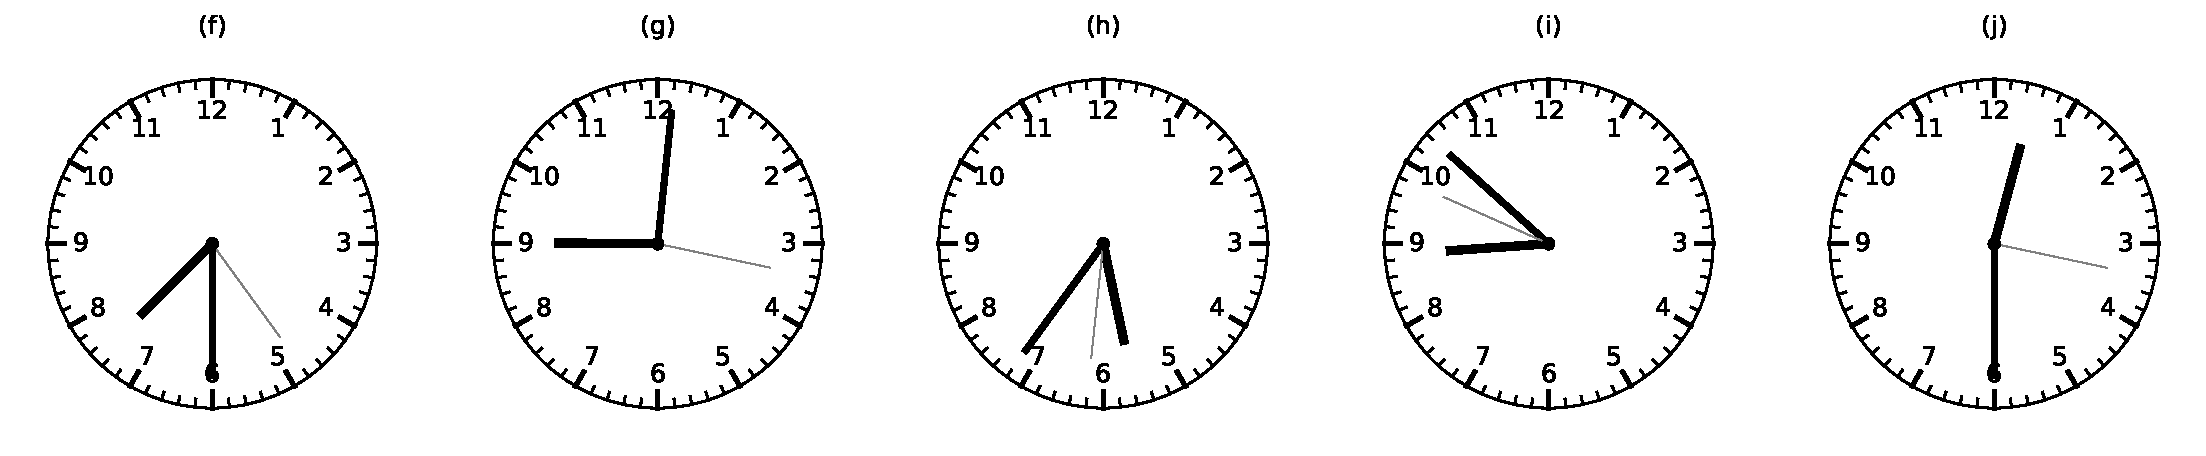
\includegraphics[width=\textwidth]{time/clocks_8_1.pdf}
\begin{enumerate}\item[(f)] \dotfill\bigskip
\item[(g)] \dotfill\bigskip
\item[(h)] \dotfill\bigskip
\item[(i)] \dotfill\bigskip
\item[(j)] \dotfill\bigskip
\end{enumerate}\clearpage
\subsection*{Problem Set \textnumero 9}

Write the time in words, to the nearest minute. For example, ``twenty-three minutes past four."

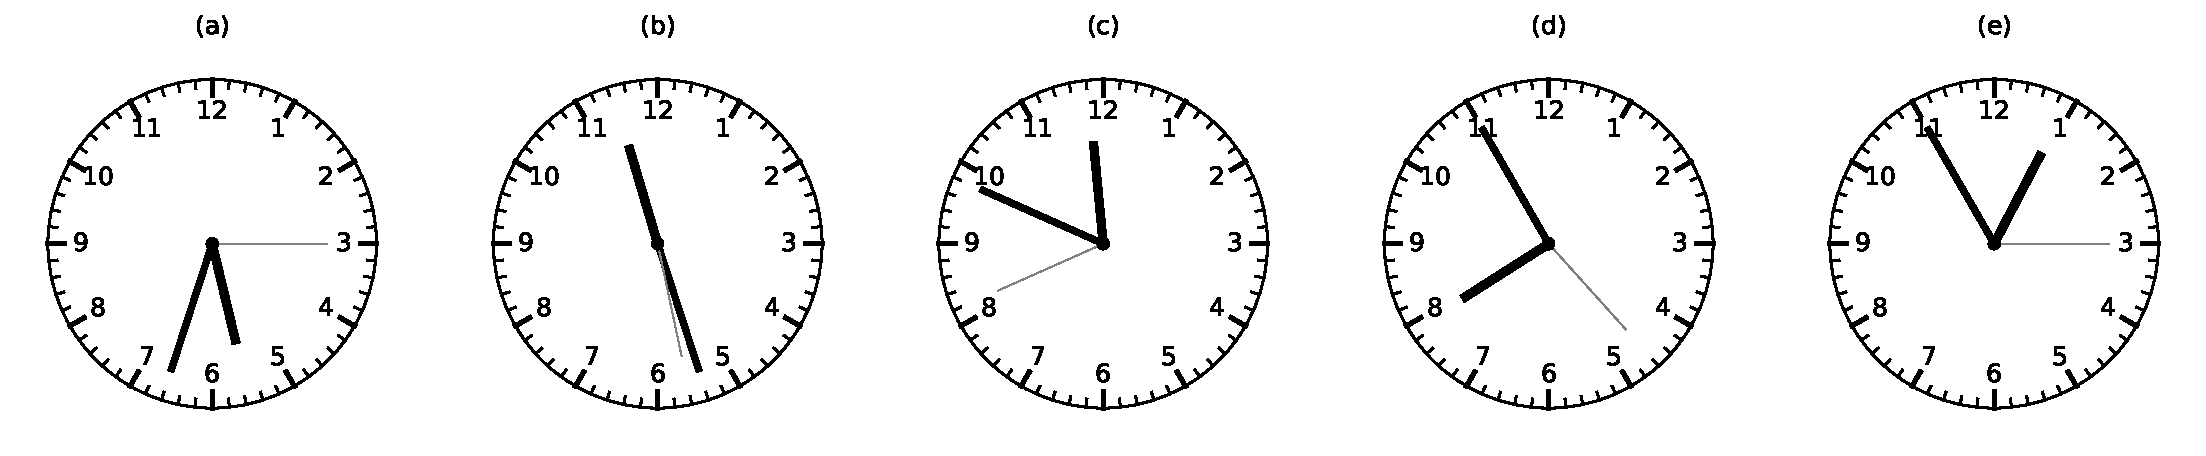
\includegraphics[width=\textwidth]{time/clocks_9_0.pdf}
\begin{enumerate}\item[(a)] \dotfill\bigskip
\item[(b)] \dotfill\bigskip
\item[(c)] \dotfill\bigskip
\item[(d)] \dotfill\bigskip
\item[(e)] \dotfill\bigskip
\end{enumerate}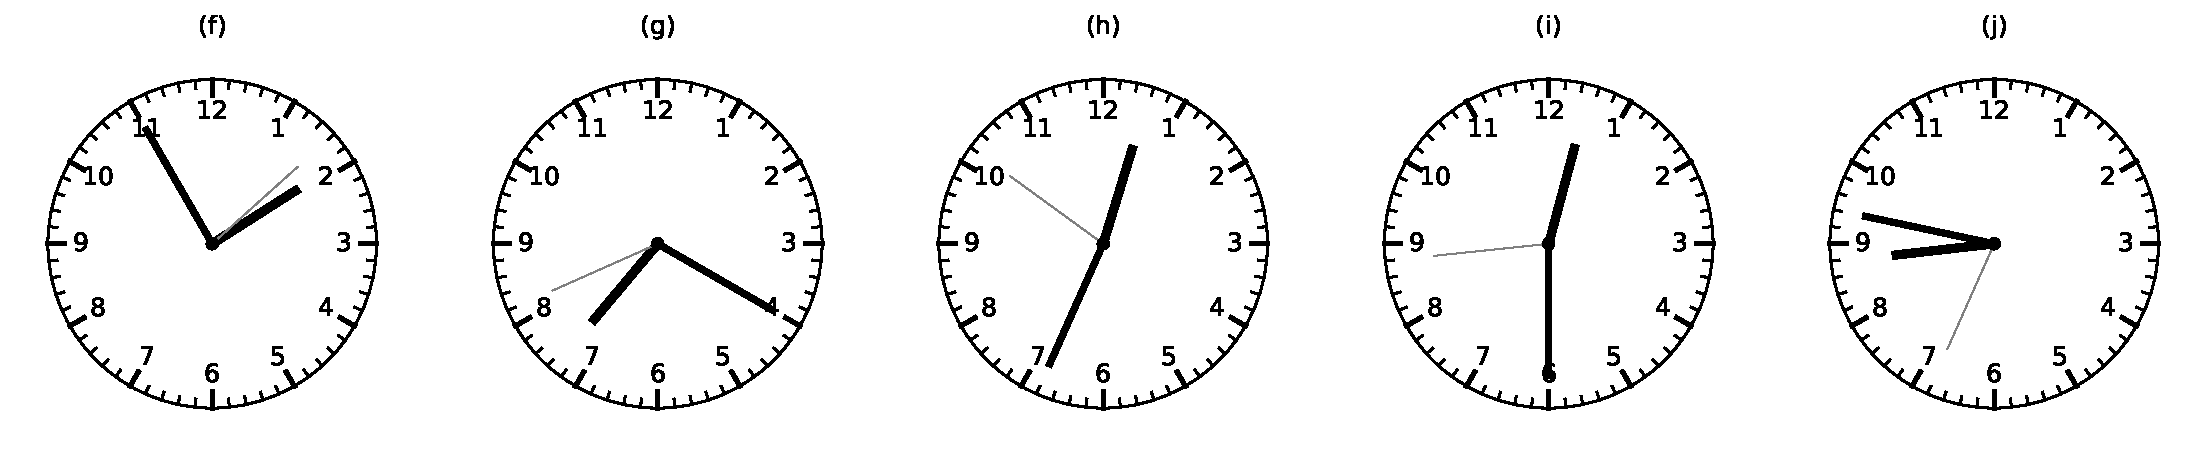
\includegraphics[width=\textwidth]{time/clocks_9_1.pdf}
\begin{enumerate}\item[(f)] \dotfill\bigskip
\item[(g)] \dotfill\bigskip
\item[(h)] \dotfill\bigskip
\item[(i)] \dotfill\bigskip
\item[(j)] \dotfill\bigskip
\end{enumerate}\clearpage
\subsection*{Problem Set \textnumero 10}

Write the time in words, to the nearest minute. For example, ``twenty-three minutes past four."

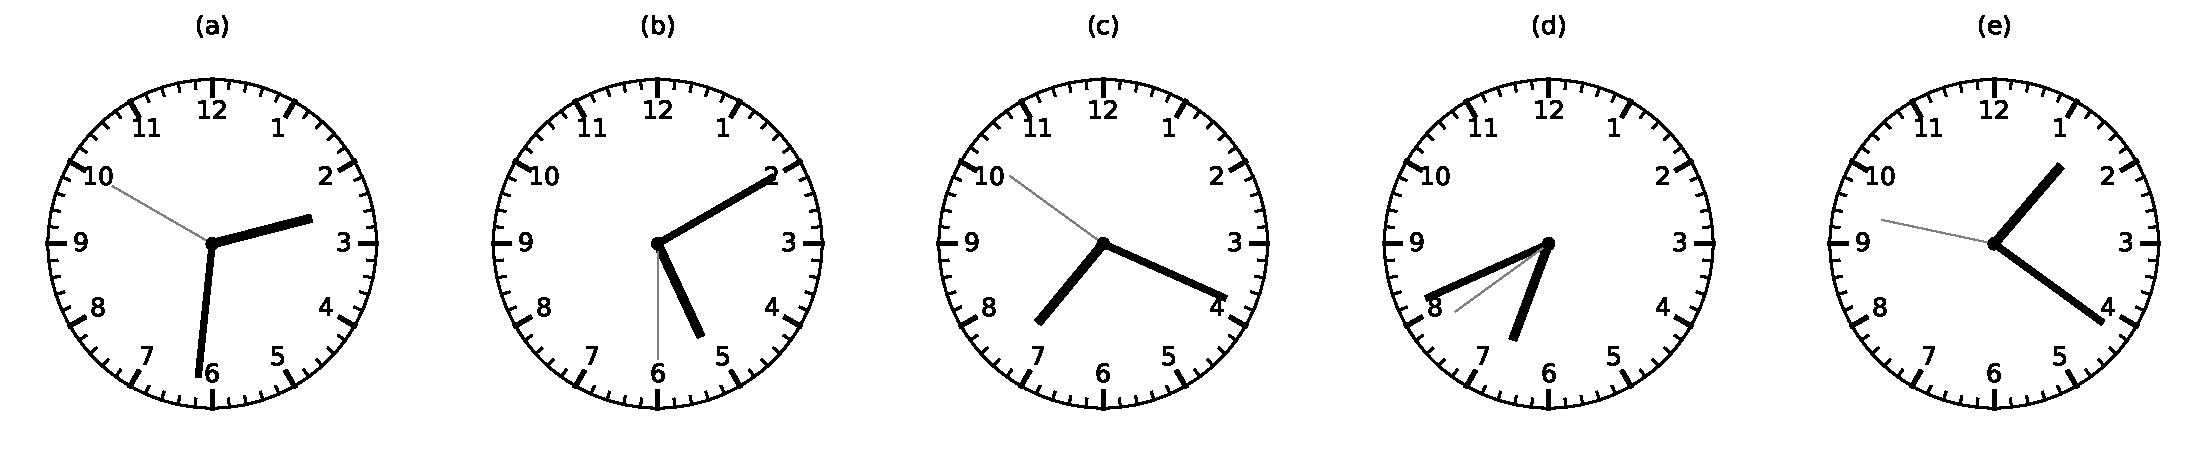
\includegraphics[width=\textwidth]{time/clocks_10_0.pdf}
\begin{enumerate}\item[(a)] \dotfill\bigskip
\item[(b)] \dotfill\bigskip
\item[(c)] \dotfill\bigskip
\item[(d)] \dotfill\bigskip
\item[(e)] \dotfill\bigskip
\end{enumerate}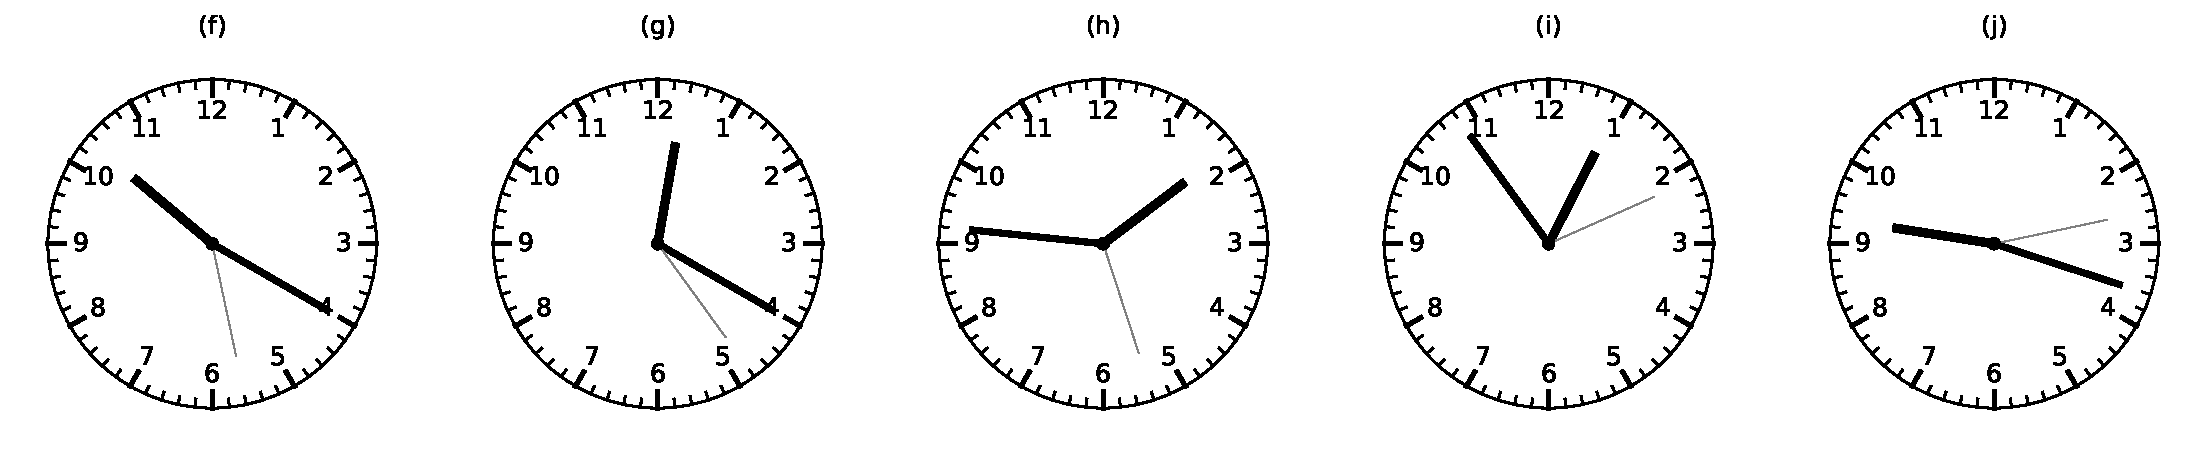
\includegraphics[width=\textwidth]{time/clocks_10_1.pdf}
\begin{enumerate}\item[(f)] \dotfill\bigskip
\item[(g)] \dotfill\bigskip
\item[(h)] \dotfill\bigskip
\item[(i)] \dotfill\bigskip
\item[(j)] \dotfill\bigskip
\end{enumerate}\clearpage\section*{Time in digital format}

\subsection*{Problem Set \textnumero 11}

Write the time in words (e.g. ``twenty-three minutes past four") and in digital format (e.g. ``04:23").

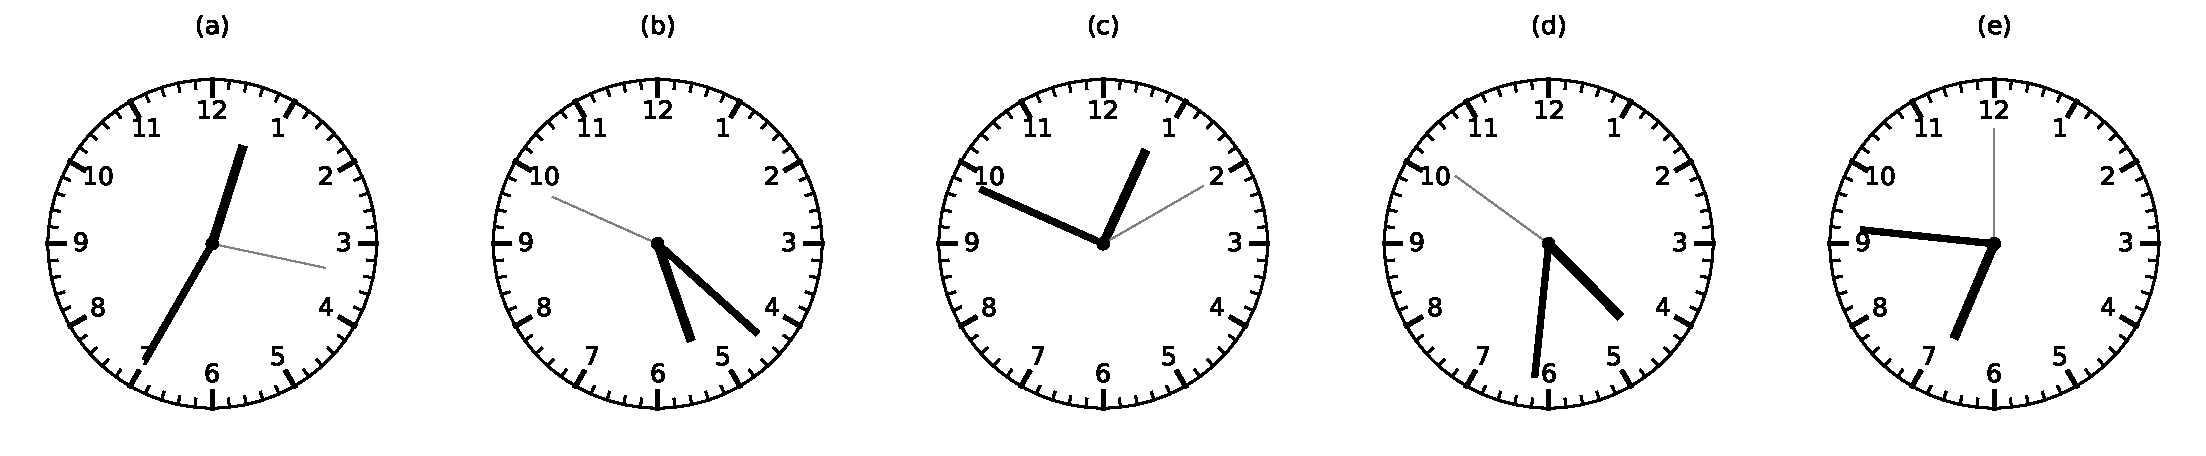
\includegraphics[width=\textwidth]{time/clocks_11_0.pdf}
\begin{enumerate}\item[(a)] \dotfill\bigskip
\item[(b)] \dotfill\bigskip
\item[(c)] \dotfill\bigskip
\item[(d)] \dotfill\bigskip
\item[(e)] \dotfill\bigskip
\end{enumerate}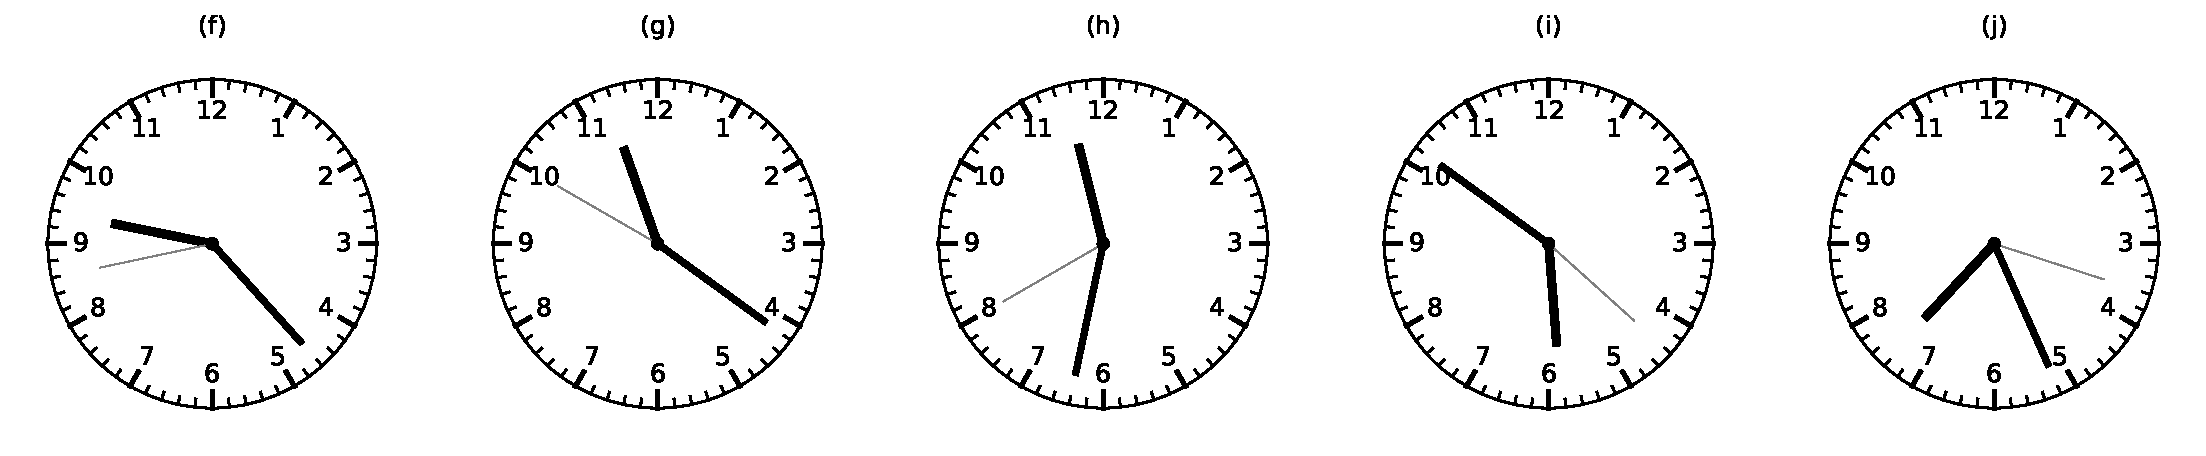
\includegraphics[width=\textwidth]{time/clocks_11_1.pdf}
\begin{enumerate}\item[(f)] \dotfill\bigskip
\item[(g)] \dotfill\bigskip
\item[(h)] \dotfill\bigskip
\item[(i)] \dotfill\bigskip
\item[(j)] \dotfill\bigskip
\end{enumerate}\clearpage
\subsection*{Problem Set \textnumero 12}

Write the time in words (e.g. ``twenty-three minutes past four") and in digital format (e.g. ``04:23").

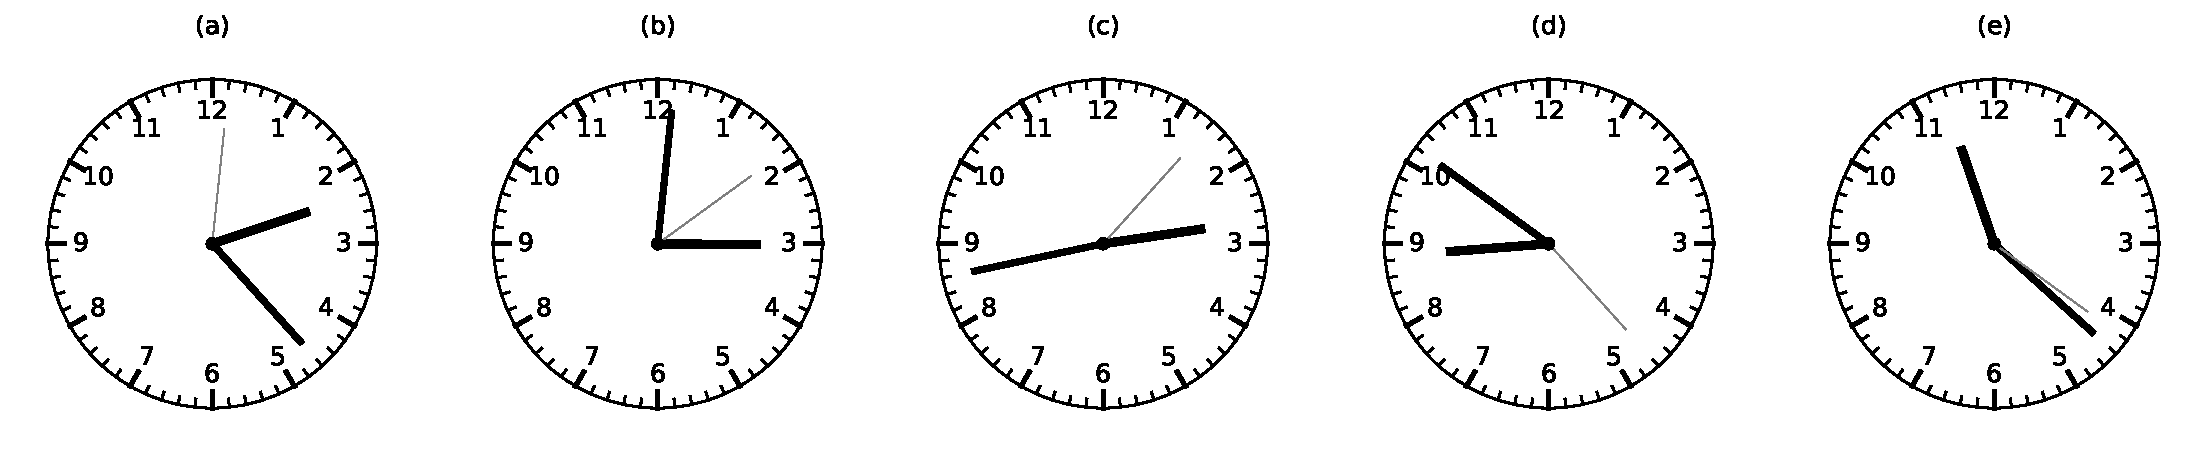
\includegraphics[width=\textwidth]{time/clocks_12_0.pdf}
\begin{enumerate}\item[(a)] \dotfill\bigskip
\item[(b)] \dotfill\bigskip
\item[(c)] \dotfill\bigskip
\item[(d)] \dotfill\bigskip
\item[(e)] \dotfill\bigskip
\end{enumerate}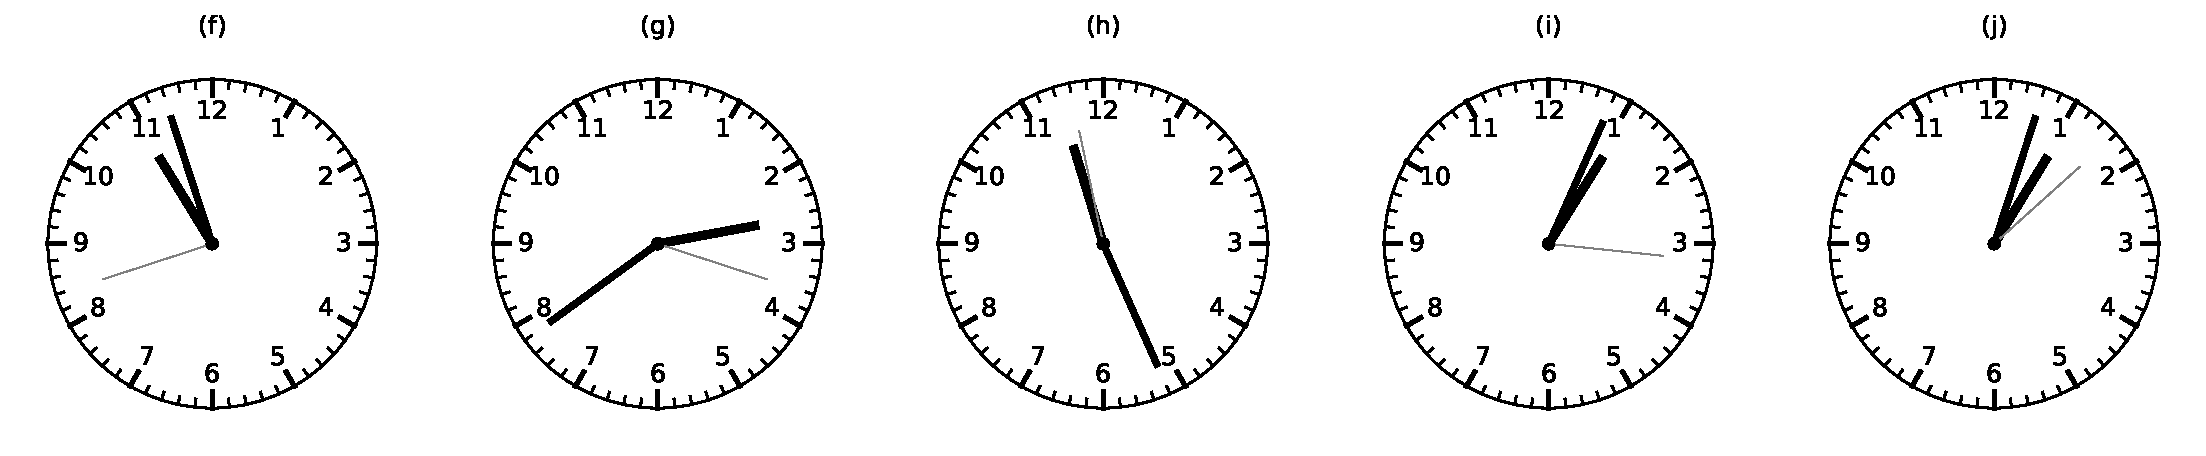
\includegraphics[width=\textwidth]{time/clocks_12_1.pdf}
\begin{enumerate}\item[(f)] \dotfill\bigskip
\item[(g)] \dotfill\bigskip
\item[(h)] \dotfill\bigskip
\item[(i)] \dotfill\bigskip
\item[(j)] \dotfill\bigskip
\end{enumerate}\clearpage
\subsection*{Problem Set \textnumero 13}

Write the time in words (e.g. ``twenty-three minutes past four") and in digital format (e.g. ``04:23").

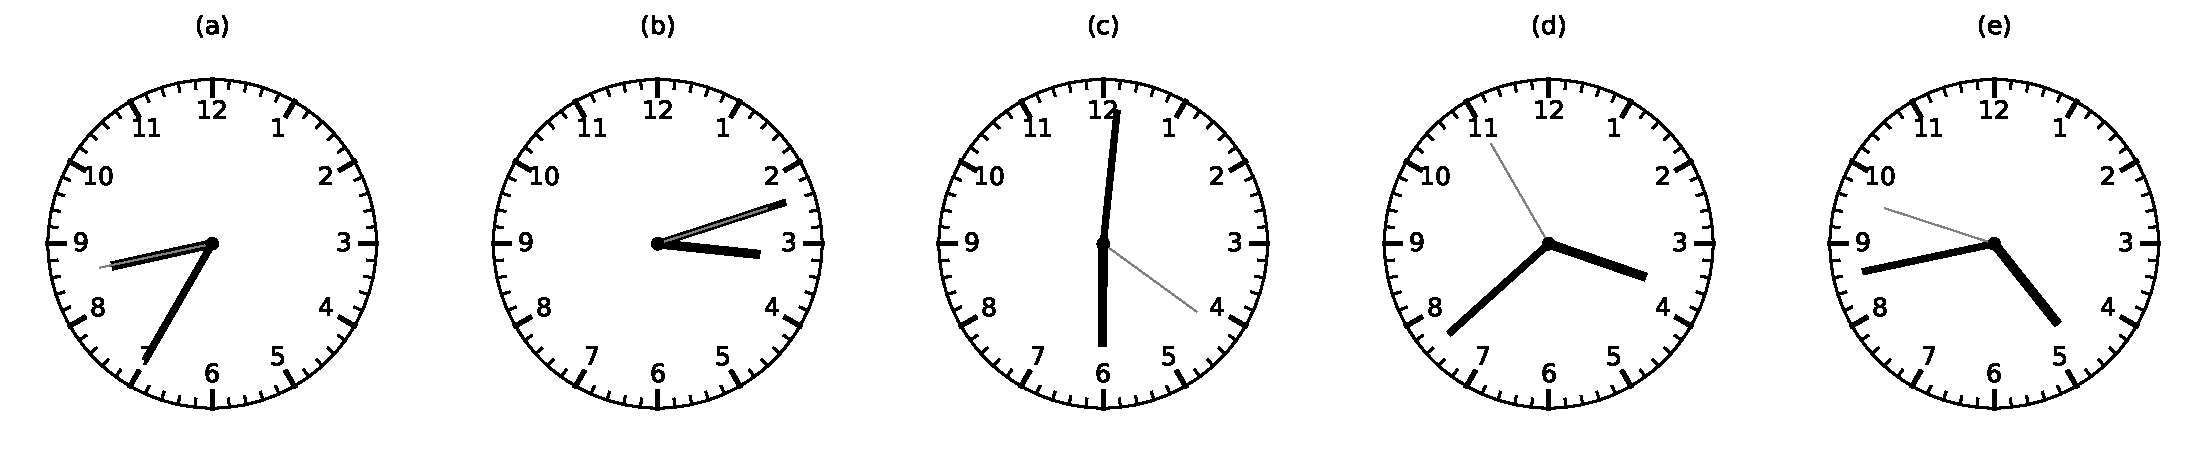
\includegraphics[width=\textwidth]{time/clocks_13_0.pdf}
\begin{enumerate}\item[(a)] \dotfill\bigskip
\item[(b)] \dotfill\bigskip
\item[(c)] \dotfill\bigskip
\item[(d)] \dotfill\bigskip
\item[(e)] \dotfill\bigskip
\end{enumerate}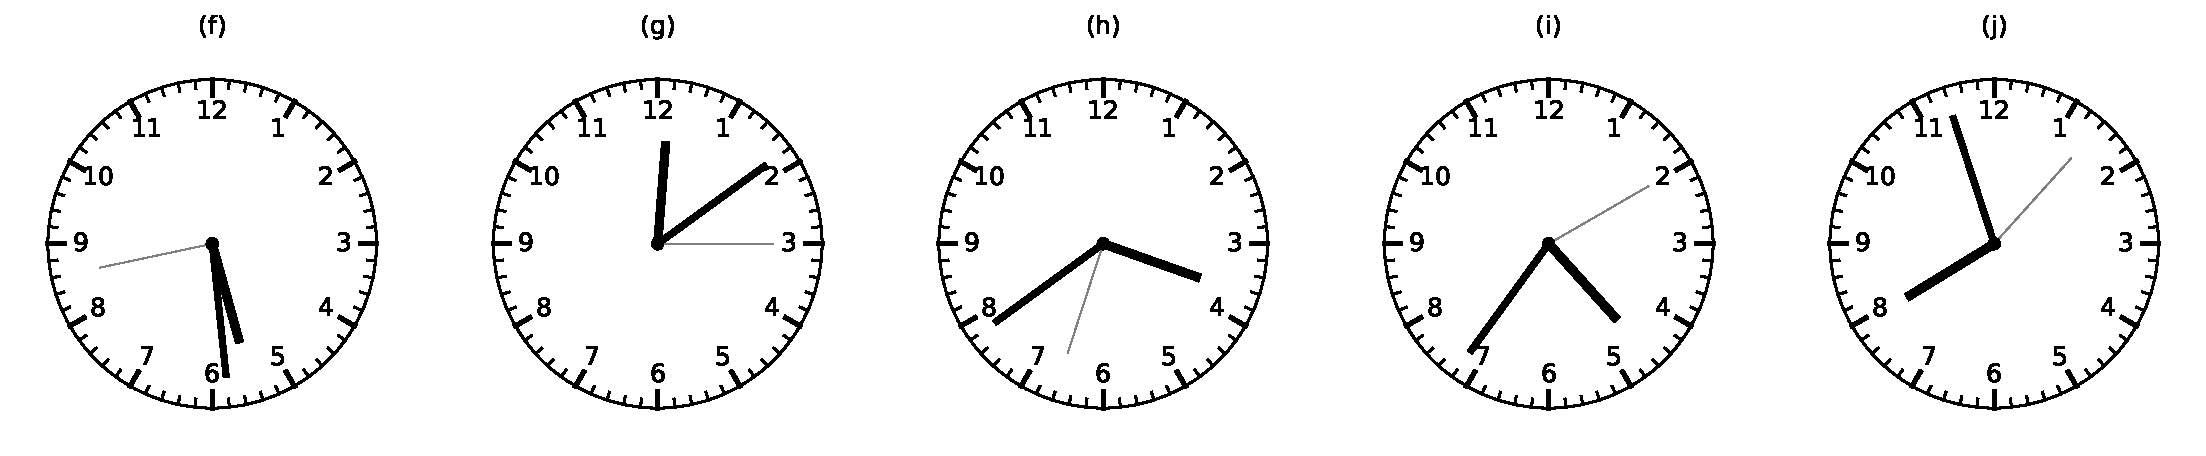
\includegraphics[width=\textwidth]{time/clocks_13_1.pdf}
\begin{enumerate}\item[(f)] \dotfill\bigskip
\item[(g)] \dotfill\bigskip
\item[(h)] \dotfill\bigskip
\item[(i)] \dotfill\bigskip
\item[(j)] \dotfill\bigskip
\end{enumerate}\clearpage
\subsection*{Problem Set \textnumero 14}

Write the time in words (e.g. ``twenty-three minutes past four") and in digital format (e.g. ``04:23").

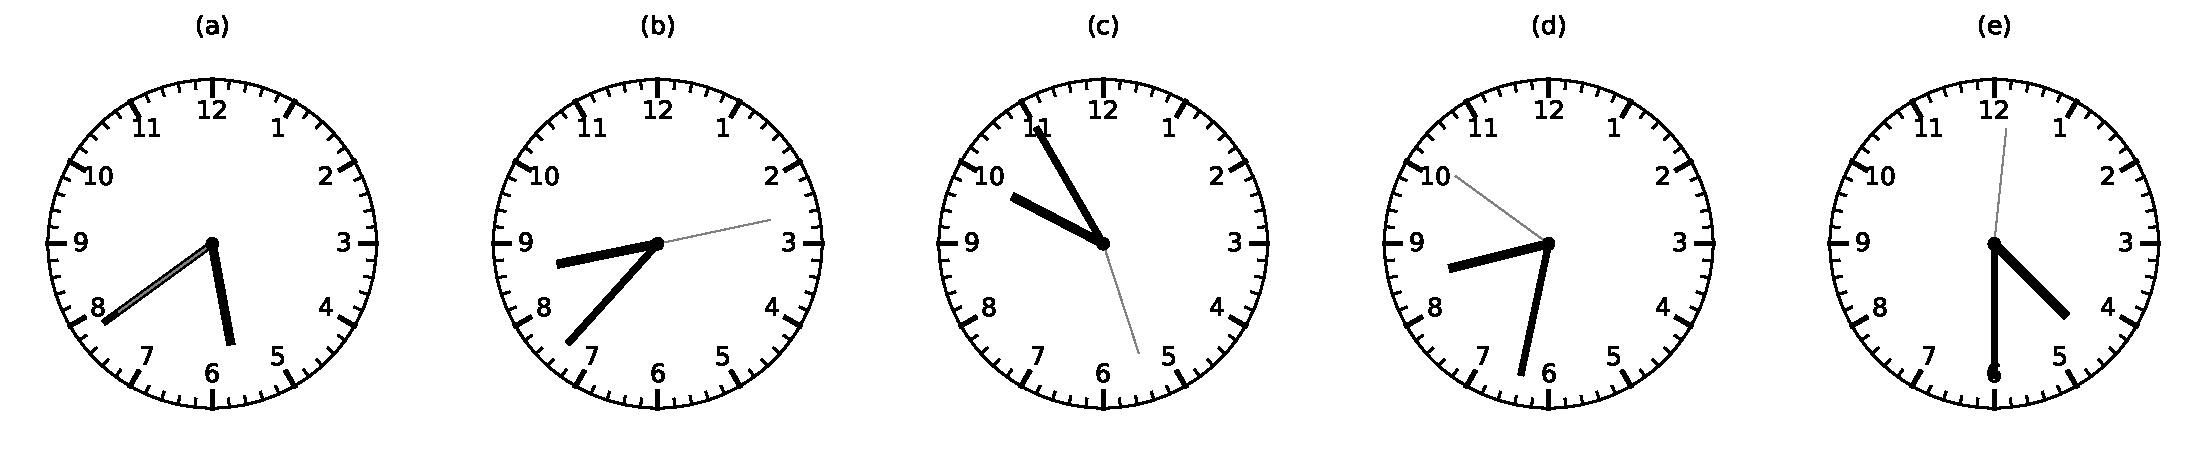
\includegraphics[width=\textwidth]{time/clocks_14_0.pdf}
\begin{enumerate}\item[(a)] \dotfill\bigskip
\item[(b)] \dotfill\bigskip
\item[(c)] \dotfill\bigskip
\item[(d)] \dotfill\bigskip
\item[(e)] \dotfill\bigskip
\end{enumerate}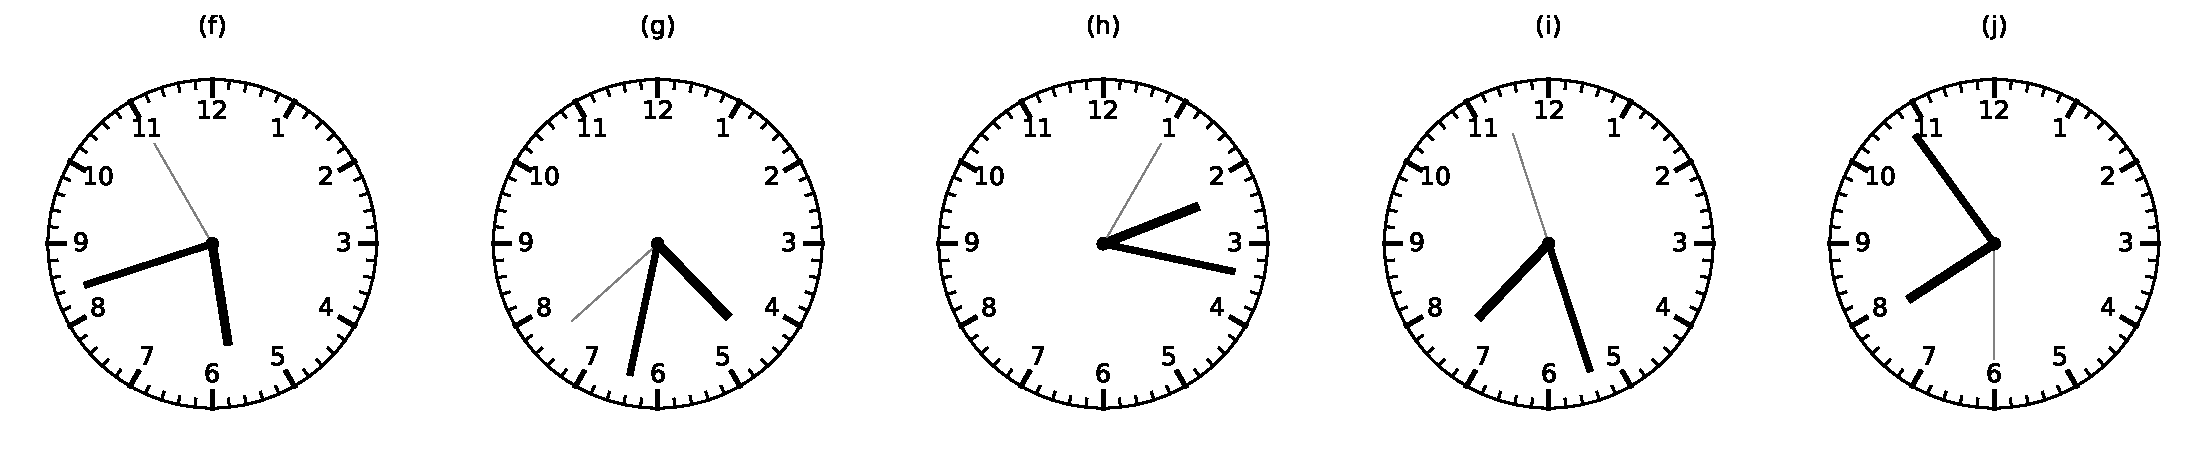
\includegraphics[width=\textwidth]{time/clocks_14_1.pdf}
\begin{enumerate}\item[(f)] \dotfill\bigskip
\item[(g)] \dotfill\bigskip
\item[(h)] \dotfill\bigskip
\item[(i)] \dotfill\bigskip
\item[(j)] \dotfill\bigskip
\end{enumerate}\clearpage
\subsection*{Problem Set \textnumero 15}

Write the time in words (e.g. ``twenty-three minutes past four") and in digital format (e.g. ``04:23").

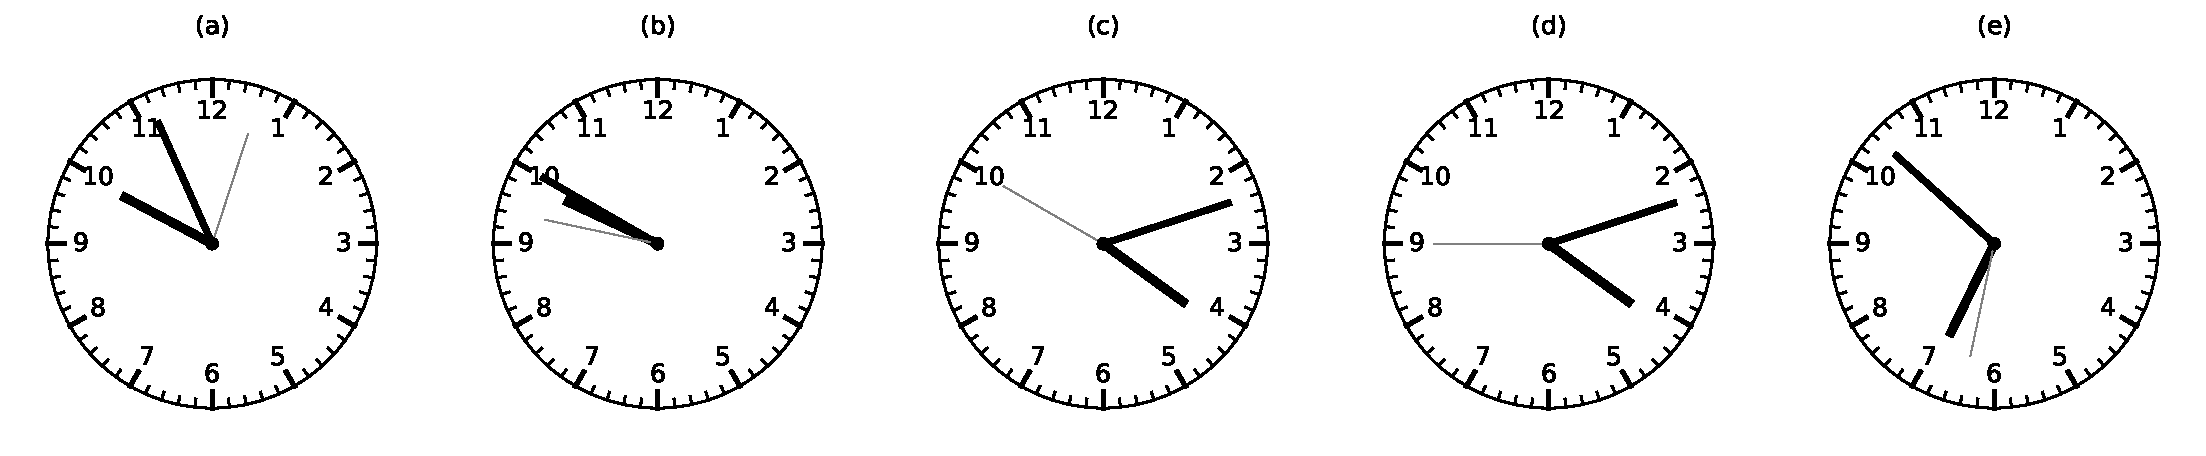
\includegraphics[width=\textwidth]{time/clocks_15_0.pdf}
\begin{enumerate}\item[(a)] \dotfill\bigskip
\item[(b)] \dotfill\bigskip
\item[(c)] \dotfill\bigskip
\item[(d)] \dotfill\bigskip
\item[(e)] \dotfill\bigskip
\end{enumerate}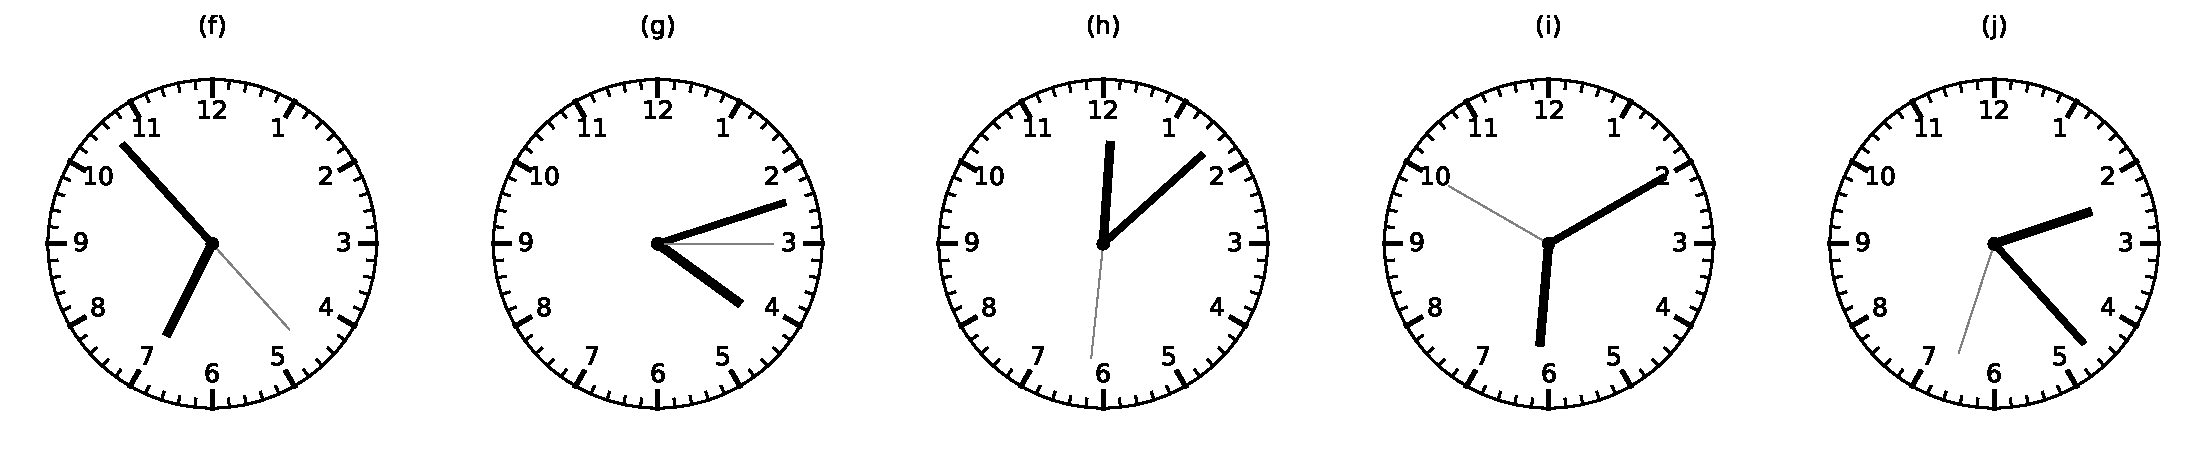
\includegraphics[width=\textwidth]{time/clocks_15_1.pdf}
\begin{enumerate}\item[(f)] \dotfill\bigskip
\item[(g)] \dotfill\bigskip
\item[(h)] \dotfill\bigskip
\item[(i)] \dotfill\bigskip
\item[(j)] \dotfill\bigskip
\end{enumerate}\end{document}